\documentclass[conference]{IEEEtran}
\usepackage[utf8]{inputenc}
\usepackage[turkish]{babel}
\usepackage{graphicx}
\usepackage{booktabs}
\usepackage{amsmath}
\usepackage{hyperref}
\usepackage{float}

\title{Makine Öğrenmesinde Özellik Seçimi Yöntemlerinin Karşılaştırmalı Analizi: Online News Popularity Veri Kümesi Üzerinde Bir Çalışma}

\author{
\IEEEauthorblockN{[Ad Soyad]}
\IEEEauthorblockA{[Öğrenci Numarası]\\
Bilgisayar Mühendisliği Bölümü\\
[Üniversite Adı]\\
Email: [email@university.edu]}
}

\begin{document}

\maketitle

% ============================================================================
% ÖZET
% ============================================================================
\begin{abstract}
Bu çalışmada, denetimli öğrenme problemlerinde özellik seçiminin sınıflandırma performansına etkisi incelenmiştir. Online News Popularity veri kümesi kullanılarak haberlerin popülerlik tahmini için bir ikili sınıflandırma modeli geliştirilmiştir. Üç farklı özellik seçimi yöntemi (Filtreleme, Sarmalayıcı ve Gömülü) uygulanarak her birinden 15 özellik seçilmiş ve Lojistik Regresyon sınıflandırıcısı ile 5-katlı çapraz doğrulama kullanılarak değerlendirilmiştir. Deneysel sonuçlar, tüm özelliklerin (59 özellik) kullanıldığı durumda \%65.62 doğruluk oranı elde edildiğini göstermiştir. Özellik seçimi yöntemleri arasında Sarmalayıcı (RFE) yöntemi 15 özellik ile \%64.64 doğruluk oranı ile en iyi performansı sergilemiştir. Optimum özellik sayısı araştırması sonucunda 30 özellik ile \%65.29 doğruluk oranına ulaşılmıştır. Sonuçlar, özellik seçiminin hesaplama süresini önemli ölçüde azaltırken performansta kabul edilebilir bir düşüşe yol açtığını ortaya koymaktadır.
\end{abstract}

\begin{IEEEkeywords}
Özellik Seçimi, Lojistik Regresyon, Filtreleme Yöntemi, RFE, Random Forest, Makine Öğrenmesi
\end{IEEEkeywords}

% ============================================================================
% GİRİŞ
% ============================================================================
\section{Giriş}

Makine öğrenmesi uygulamalarında veri kümelerinin boyutu ve karmaşıklığı sürekli artmaktadır. Yüksek boyutlu veri kümeleri, modelin eğitim süresini uzatmakta, aşırı öğrenme (overfitting) riskini artırmakta ve yorumlanabilirliği azaltmaktadır \cite{guyon2003introduction}. Bu nedenle, özellik seçimi makine öğrenmesi iş akışının kritik bir bileşeni haline gelmiştir.

Bu çalışmanın amacı, farklı özellik seçimi yöntemlerinin sınıflandırma performansı üzerindeki etkisini incelemektir. Bu amaçla, Mashable haber sitesinden toplanan Online News Popularity veri kümesi kullanılmıştır. Veri kümesi, 39.644 haber makalesinin 59 özelliğini içermekte olup hedef değişken olarak paylaşım sayısı kullanılmaktadır.

Çalışma kapsamında üç ana özellik seçimi kategorisi değerlendirilmiştir:
\begin{itemize}
    \item \textbf{Filtreleme Yöntemi:} Pearson korelasyonu kullanarak özellikler arası ilişkiyi analiz eder.
    \item \textbf{Sarmalayıcı Yöntem:} Recursive Feature Elimination (RFE) ile iteratif özellik eleme yapar.
    \item \textbf{Gömülü Yöntem:} Random Forest özellik önem skorlarını kullanır.
\end{itemize}

Çalışmanın geri kalanı şu şekilde organize edilmiştir: Bölüm 2'de deneysel metodoloji ve sonuçlar sunulmuş, Bölüm 3'te elde edilen bulgular tartışılmıştır.

% ============================================================================
% DENEYSEL ANALİZ
% ============================================================================
\section{Deneysel Analiz}

\subsection{Veri Kümesi}

Online News Popularity veri kümesi, UCI Machine Learning Repository'den elde edilmiştir \cite{fernandes2015proactive}. Veri kümesi, Mashable web sitesinde yayınlanan 39.644 haber makalesinin istatistiksel özelliklerini içermektedir. Özellikler arasında:

\begin{itemize}
    \item Metin istatistikleri (kelime sayısı, benzersiz token oranı)
    \item Bağlantı bilgileri (hiper bağlantı sayısı, görsel sayısı)
    \item Anahtar kelime metrikleri
    \item Yayın zamanı bilgileri (haftanın günü, hafta sonu)
    \item LDA konu modelleme skorları
    \item Duygu analizi metrikleri
\end{itemize}

\subsection{Veri Ön İşleme}

Veri ön işleme aşamasında aşağıdaki adımlar uygulanmıştır:

\begin{enumerate}
    \item \textbf{Özellik Kaldırma:} Ayırt edici bilgi içermeyen \texttt{url} sütunu kaldırılmıştır.
    \item \textbf{Hedef Değişken Dönüşümü:} Paylaşım sayısı (\texttt{shares}) için medyan değeri olan 1400 eşik olarak belirlenmiş ve ikili sınıflandırma problemi oluşturulmuştur:
    \begin{equation}
        y = \begin{cases} 
        1 & \text{eğer } shares \geq 1400 \\
        0 & \text{diğer durumda}
        \end{cases}
    \end{equation}
    \item \textbf{Veri Bölme:} Veri kümesi \%80 eğitim (31.715 örnek) ve \%20 test (7.929 örnek) olarak stratified örnekleme ile bölünmüştür.
    \item \textbf{Normalizasyon:} Z-score standartlaştırması uygulanmıştır.
\end{enumerate}

Hedef değişken dağılımı Tablo \ref{tab:target_dist}'te gösterilmiştir.

\begin{table}[H]
\centering
\caption{Hedef Değişken Dağılımı}
\label{tab:target_dist}
\begin{tabular}{lcc}
\toprule
\textbf{Sınıf} & \textbf{Örnek Sayısı} & \textbf{Oran (\%)} \\
\midrule
Popüler (1) & 21.154 & 53.36 \\
Popüler Değil (0) & 18.490 & 46.64 \\
\midrule
\textbf{Toplam} & 39.644 & 100.00 \\
\bottomrule
\end{tabular}
\end{table}

\subsection{Özellik Seçimi Yöntemleri}

\subsubsection{Filtreleme Yöntemi (Pearson Korelasyonu)}

Filtreleme yönteminde, öncelikle özellikler arası korelasyon matrisi hesaplanmış ve 0.8'den yüksek korelasyona sahip özellik çiftlerinden biri elenmiştir (multicollinearity azaltma). Ardından, hedef değişken ile korelasyonu en yüksek 15 özellik seçilmiştir. Seçilen özellikler Tablo \ref{tab:filter_features}'de listelenmiştir.

\begin{table}[H]
\centering
\caption{Filtreleme Yöntemi ile Seçilen Özellikler}
\label{tab:filter_features}
\begin{tabular}{clc}
\toprule
\textbf{Sıra} & \textbf{Özellik} & \textbf{Korelasyon} \\
\midrule
1 & LDA\_02 & 0.1603 \\
2 & kw\_avg\_avg & 0.1562 \\
3 & is\_weekend & 0.1387 \\
4 & data\_channel\_is\_entertainment & 0.1129 \\
5 & data\_channel\_is\_socmed & 0.1103 \\
6 & weekday\_is\_saturday & 0.1079 \\
7 & data\_channel\_is\_tech & 0.1044 \\
8 & LDA\_04 & 0.0960 \\
9 & num\_hrefs & 0.0921 \\
10 & kw\_min\_avg & 0.0908 \\
11 & weekday\_is\_sunday & 0.0821 \\
12 & LDA\_01 & 0.0789 \\
13 & num\_keywords & 0.0762 \\
14 & global\_sentiment\_polarity & 0.0699 \\
15 & global\_subjectivity & 0.0682 \\
\bottomrule
\end{tabular}
\end{table}

\subsubsection{Sarmalayıcı Yöntem (RFE)}

Recursive Feature Elimination (RFE) yöntemi, Lojistik Regresyon sınıflandırıcısı ile birlikte kullanılmıştır \cite{guyon2002gene}. RFE, her iterasyonda en düşük önem skoruna sahip özelliği eleyerek 15 özellik kalana kadar devam etmiştir.

Seçilen özellikler: \texttt{n\_non\_stop\_words}, \texttt{n\_non\_stop\_unique\_tokens}, \texttt{data\_channel\_is\_socmed}, \texttt{data\_channel\_is\_tech}, \texttt{kw\_min\_min}, \texttt{kw\_max\_min}, \texttt{kw\_avg\_min}, \texttt{kw\_avg\_max}, \texttt{kw\_min\_avg}, \texttt{kw\_max\_avg}, \texttt{kw\_avg\_avg}, \texttt{is\_weekend}, \texttt{LDA\_01}, \texttt{LDA\_02}, \texttt{LDA\_03}.

\subsubsection{Gömülü Yöntem (Random Forest)}

Random Forest sınıflandırıcısı (100 ağaç) eğitilerek özellik önem skorları hesaplanmıştır \cite{breiman2001random}. En yüksek önem skoruna sahip 15 özellik seçilmiştir.

En önemli üç özellik: \texttt{kw\_avg\_avg} (0.0697), \texttt{kw\_max\_avg} (0.0630), \texttt{self\_reference\_min\_shares} (0.0568).

\subsubsection{Özellik Karşılaştırması}

Üç yöntemde de ortak seçilen özellikler Tablo \ref{tab:common_features}'de gösterilmiştir.

\begin{table}[H]
\centering
\caption{Tüm Yöntemlerde Ortak Özellikler}
\label{tab:common_features}
\begin{tabular}{l}
\toprule
\textbf{Ortak Özellikler (5 adet)} \\
\midrule
is\_weekend \\
kw\_avg\_avg \\
kw\_min\_avg \\
LDA\_01 \\
LDA\_02 \\
\bottomrule
\end{tabular}
\end{table}

Bu özelliklerin tüm yöntemlerde seçilmesi, haberlerin popülerliğini tahmin etmede anahtar kelime metrikleri, LDA konu skorları ve hafta sonu yayın zamanlamasının önemini göstermektedir.

\subsection{Model Eğitimi ve Değerlendirme}

\subsubsection{Regularizasyon Parametresi Optimizasyonu}

Aşırı öğrenmeyi önlemek için Lojistik Regresyon'un C (regularizasyon) parametresi 5-katlı çapraz doğrulama ile optimize edilmiştir. Test edilen değerler ve sonuçları Tablo \ref{tab:regularization}'de sunulmuştur.

\begin{table}[H]
\centering
\caption{Regularizasyon Parametresi Arama Sonuçları}
\label{tab:regularization}
\begin{tabular}{cc}
\toprule
\textbf{C Değeri} & \textbf{CV Accuracy} \\
\midrule
0.001 & 0.6499 $\pm$ 0.0046 \\
0.01 & 0.6521 $\pm$ 0.0042 \\
0.1 & 0.6523 $\pm$ 0.0028 \\
1.0 & 0.6523 $\pm$ 0.0030 \\
10.0 & 0.6524 $\pm$ 0.0022 \\
\textbf{100.0} & \textbf{0.6525 $\pm$ 0.0023} \\
\bottomrule
\end{tabular}
\end{table}

En iyi C değeri 100 olarak belirlenmiştir. Düşük C değerlerinde (güçlü regularizasyon) performans düşüşü gözlemlenmiştir, bu da modelin yetersiz öğrenme (underfitting) durumunda olduğunu göstermektedir.

\subsubsection{Çapraz Doğrulama Sonuçları}

5-katlı stratified çapraz doğrulama kullanılarak tüm yöntemler değerlendirilmiştir. Eğitim ve doğrulama sonuçları Tablo \ref{tab:cv_results}'de özetlenmiştir.

\begin{table}[H]
\centering
\caption{5-Katlı Çapraz Doğrulama Sonuçları}
\label{tab:cv_results}
\begin{tabular}{lcccc}
\toprule
\textbf{Yöntem} & \textbf{Accuracy} & \textbf{F1-Score} & \textbf{Precision} & \textbf{Recall} \\
\midrule
Tüm Özellikler & 0.6525 & 0.6820 & 0.6665 & 0.6985 \\
Filtreleme & 0.6431 & 0.6763 & 0.6555 & 0.6985 \\
Sarmalayıcı & 0.6481 & 0.6791 & 0.6616 & 0.6976 \\
Gömülü & 0.6386 & 0.6788 & 0.6457 & 0.7156 \\
\bottomrule
\end{tabular}
\end{table}

\subsubsection{Test Seti Sonuçları}

Eğitilmiş modeller, ayrı tutulan \%20 test seti üzerinde değerlendirilmiştir. Sonuçlar Tablo \ref{tab:test_results}'de sunulmuştur.

\begin{table}[H]
\centering
\caption{Test Seti Performans Sonuçları}
\label{tab:test_results}
\begin{tabular}{lccccc}
\toprule
\textbf{Yöntem} & \textbf{Özellik} & \textbf{Accuracy} & \textbf{F1-Score} & \textbf{Eğitim} \\
 & \textbf{Sayısı} & & & \textbf{Süresi} \\
\midrule
Tüm Özellikler & 59 & \textbf{0.6562} & \textbf{0.6849} & 3.49s \\
Filtreleme & 15 & 0.6436 & 0.6776 & 0.54s \\
Sarmalayıcı & 15 & 0.6464 & 0.6779 & 1.19s \\
Gömülü & 15 & 0.6396 & 0.6823 & 0.79s \\
Optimal (RFE) & 30 & 0.6529 & 0.6827 & 2.06s \\
\bottomrule
\end{tabular}
\end{table}

\subsubsection{Optimum Özellik Sayısı Araştırması}

En başarılı özellik seçimi yöntemi olan Sarmalayıcı (RFE) kullanılarak optimum özellik sayısı araştırılmıştır. 5'ten 30'a kadar farklı özellik sayıları test edilmiştir.

\begin{table}[H]
\centering
\caption{Optimum Özellik Sayısı Araştırması}
\label{tab:optimal_search}
\begin{tabular}{cc}
\toprule
\textbf{Özellik Sayısı} & \textbf{CV Accuracy} \\
\midrule
5 & 0.6096 $\pm$ 0.0060 \\
10 & 0.6410 $\pm$ 0.0072 \\
15 & 0.6486 $\pm$ 0.0081 \\
20 & 0.6520 $\pm$ 0.0071 \\
25 & 0.6516 $\pm$ 0.0072 \\
\textbf{30} & \textbf{0.6520 $\pm$ 0.0054} \\
\bottomrule
\end{tabular}
\end{table}

Optimum özellik sayısı 30 olarak belirlenmiş ve bu özelliklerle \%65.29 test doğruluğu elde edilmiştir.

\subsubsection{Karışıklık Matrisi}

En başarılı yöntem (Tüm Özellikler) için karışıklık matrisi Tablo \ref{tab:confusion}'de gösterilmiştir.

\begin{table}[H]
\centering
\caption{Tüm Özellikler Yöntemi için Karışıklık Matrisi}
\label{tab:confusion}
\begin{tabular}{lcc}
\toprule
& \textbf{Tahmin: 0} & \textbf{Tahmin: 1} \\
\midrule
\textbf{Gerçek: 0} & 2241 (TN) & 1457 (FP) \\
\textbf{Gerçek: 1} & 1269 (FN) & 2962 (TP) \\
\bottomrule
\end{tabular}
\end{table}

Karışıklık matrisinden hesaplanan metrikler:
\begin{itemize}
    \item \textbf{Doğruluk (Accuracy):} $(2241 + 2962) / 7929 = 0.6562$
    \item \textbf{Kesinlik (Precision):} $2962 / (2962 + 1457) = 0.6703$
    \item \textbf{Duyarlılık (Recall):} $2962 / (2962 + 1269) = 0.7001$
    \item \textbf{F1-Skoru:} $2 \times (0.6703 \times 0.7001) / (0.6703 + 0.7001) = 0.6849$
\end{itemize}

\begin{figure}[H]
\centering
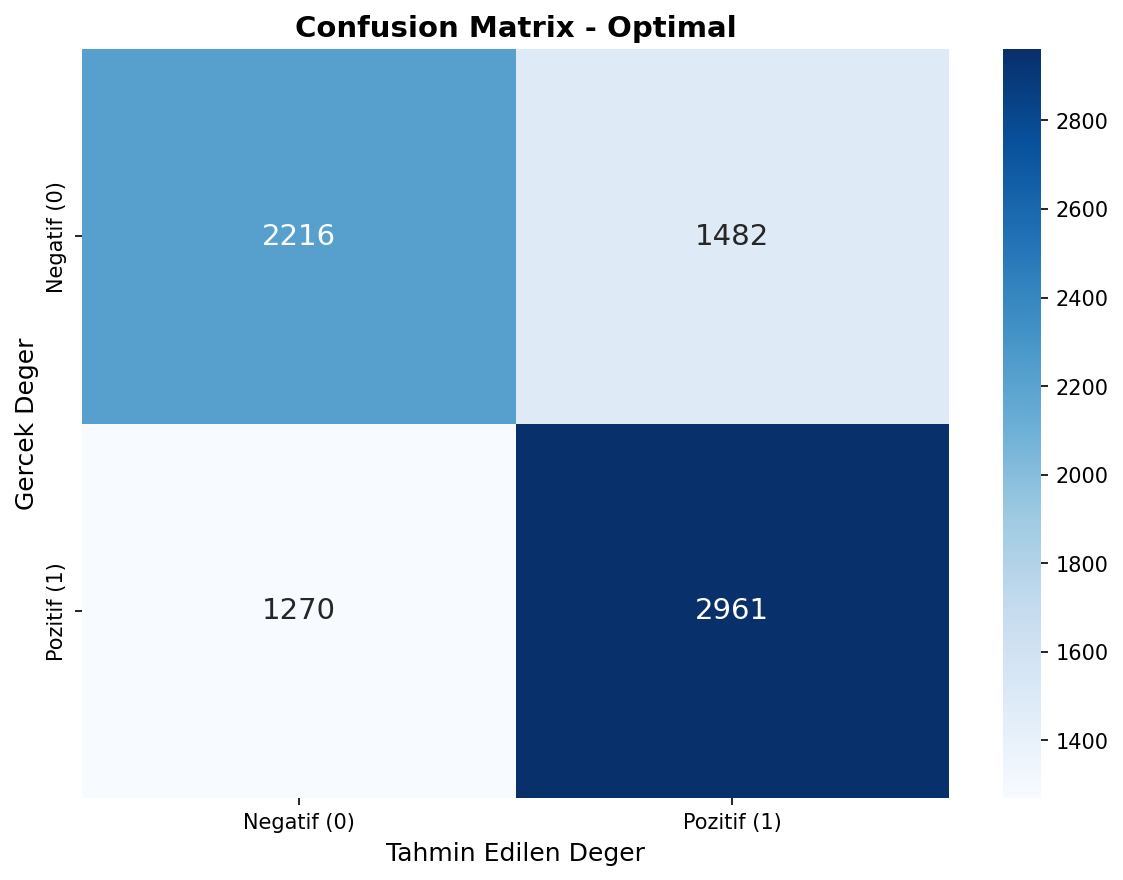
\includegraphics[width=0.45\textwidth]{../results/confusion_matrix.png}
\caption{En başarılı yöntem için karışıklık matrisi görselleştirmesi}
\label{fig:confusion}
\end{figure}

\begin{figure}[H]
\centering
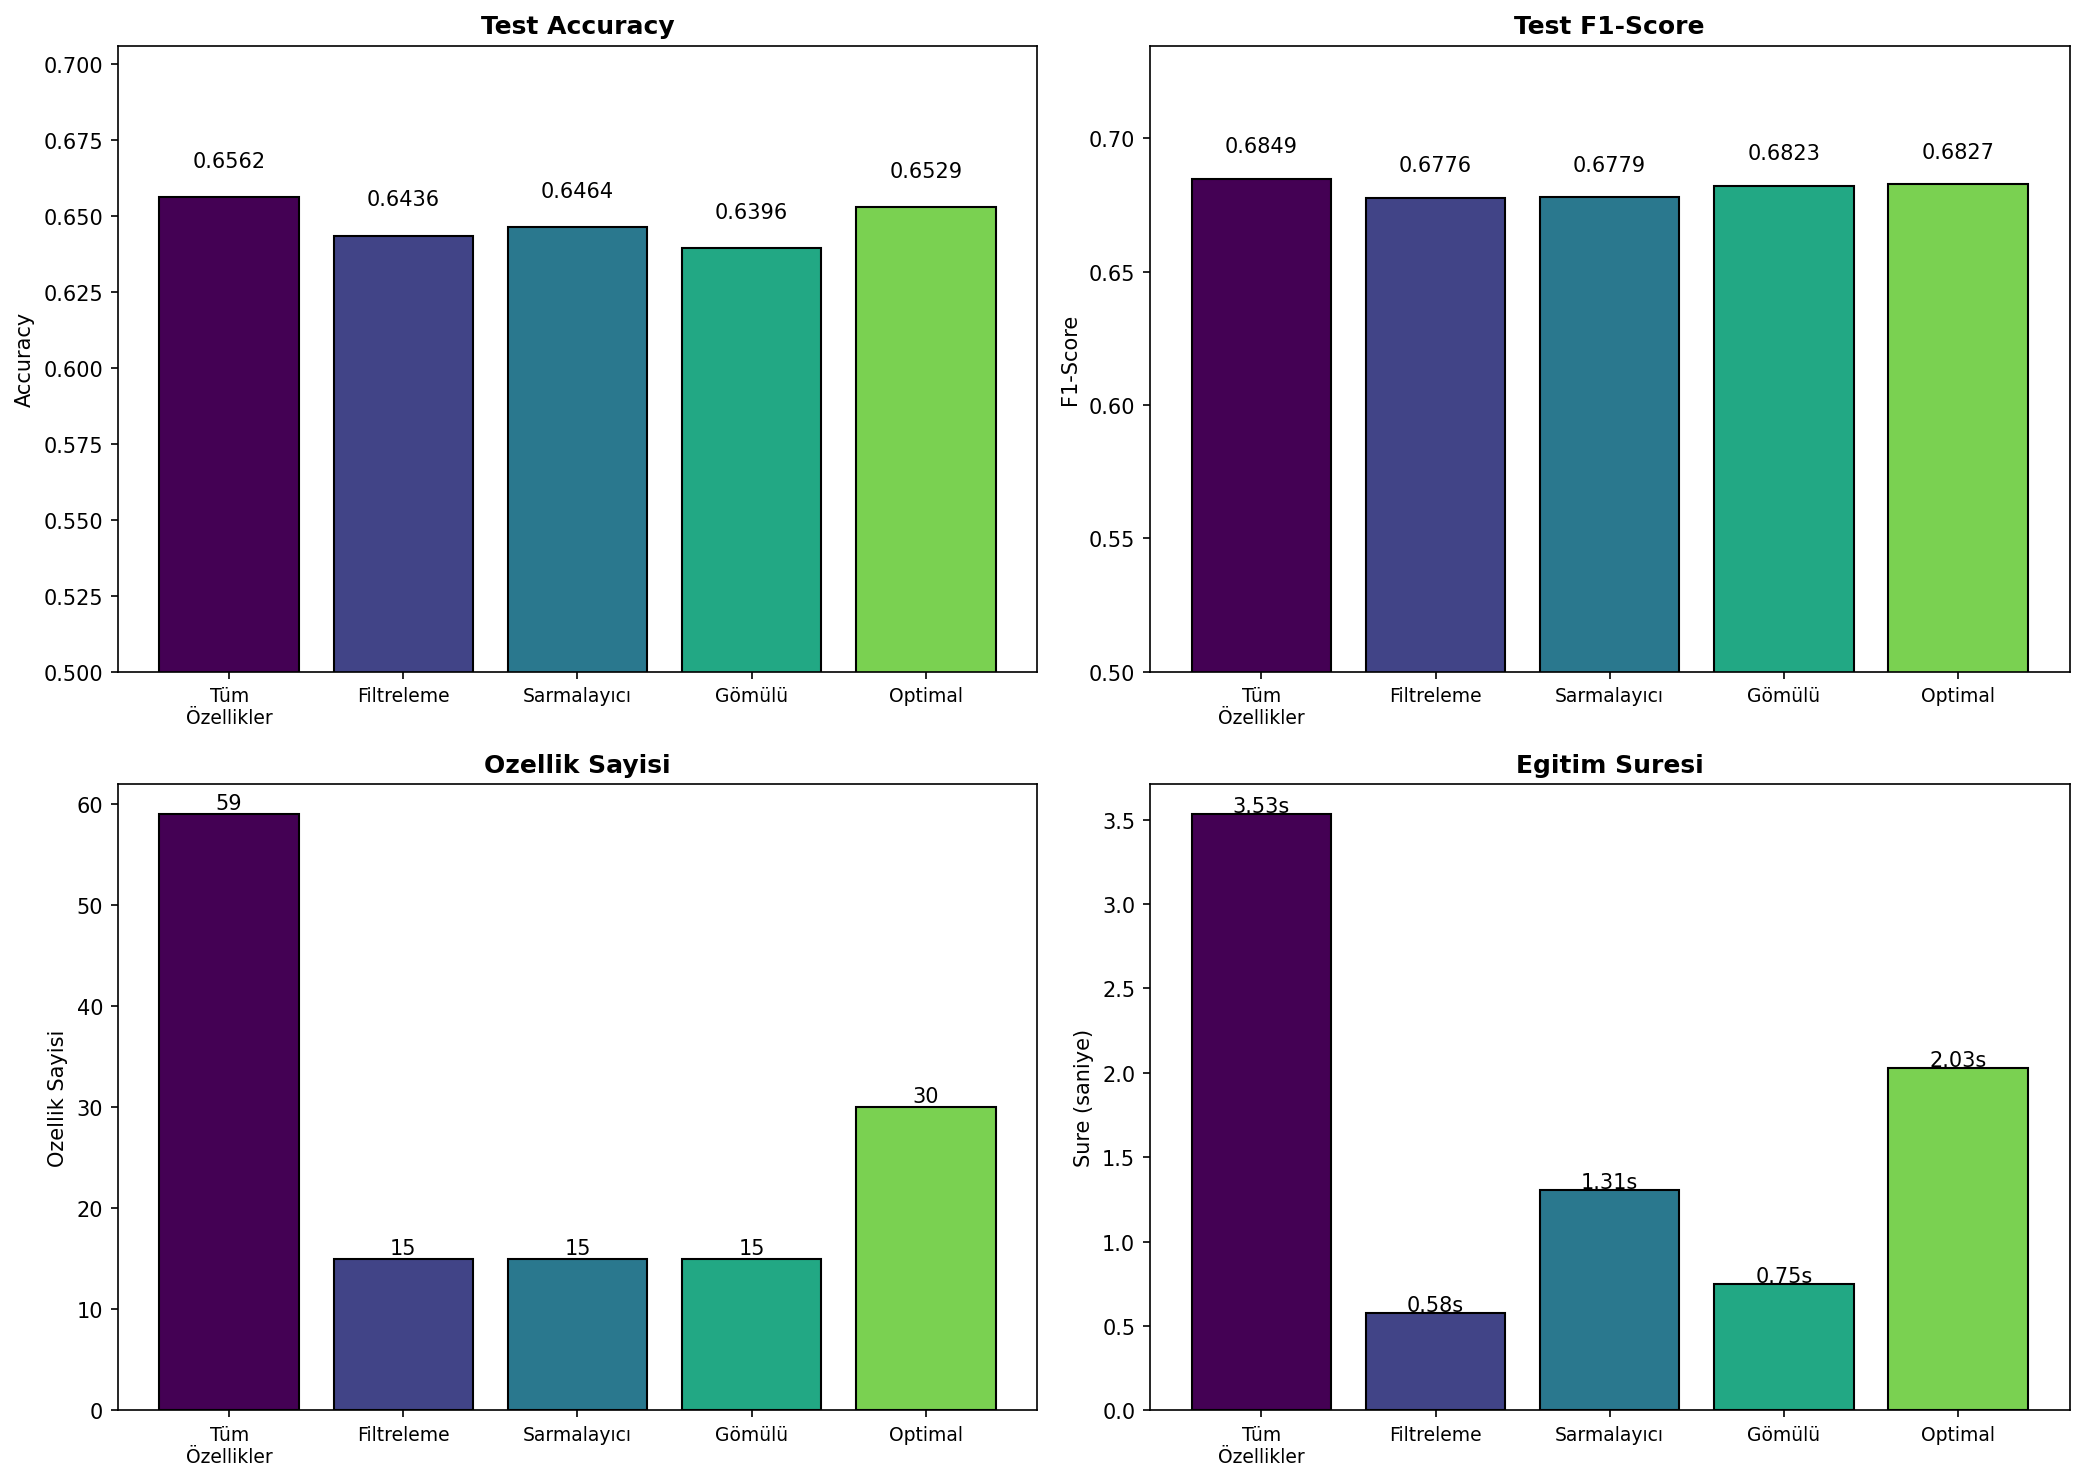
\includegraphics[width=0.48\textwidth]{../results/results_comparison.png}
\caption{Yöntemlerin performans karşılaştırması}
\label{fig:comparison}
\end{figure}

% ============================================================================
% SONUÇ
% ============================================================================
\section{Sonuç}

Bu çalışmada, Online News Popularity veri kümesi üzerinde üç farklı özellik seçimi yöntemi (Filtreleme, Sarmalayıcı ve Gömülü) karşılaştırmalı olarak değerlendirilmiştir. Deneysel sonuçlar, tüm 59 özelliğin kullanıldığı durumda \%65.62 ile en yüksek doğruluk oranına ulaşıldığını göstermiştir. Ancak özellik seçimi yöntemleri, sadece 15 özellik ile \%64-65 arasında performans sergileyerek hesaplama süresini önemli ölçüde azaltmıştır (3.49s'den 0.54-1.19s'ye).

Özellik seçimi yöntemleri arasında Sarmalayıcı (RFE) yöntemi en iyi performansı (\%64.64) göstermiştir. Bu yöntem, model performansını doğrudan optimize ettiği için diğer yöntemlere göre daha tutarlı sonuçlar üretmiştir. Optimum özellik sayısı araştırması sonucunda 30 özelliğin \%65.29 doğruluk ile en iyi dengeyi sağladığı belirlenmiştir.

Tüm yöntemlerde ortak olarak seçilen 5 özellik (\texttt{is\_weekend}, \texttt{kw\_avg\_avg}, \texttt{kw\_min\_avg}, \texttt{LDA\_01}, \texttt{LDA\_02}), haber popülerliğini etkileyen anahtar faktörleri ortaya koymuştur. Bu bulgular, anahtar kelime optimizasyonu ve yayın zamanlamasının haber paylaşımlarını artırmada kritik rol oynadığını göstermektedir.

Sonuç olarak, özellik seçimi model yorumlanabilirliğini artırırken hesaplama maliyetini düşürmekte, ancak performansta küçük bir düşüşe neden olmaktadır. Uygulama gereksinimlerine göre bu denge dikkate alınmalıdır.

% ============================================================================
% KAYNAKLAR
% ============================================================================
\begin{thebibliography}{9}

\bibitem{guyon2003introduction}
I. Guyon and A. Elisseeff, ``An introduction to variable and feature selection,'' \textit{Journal of Machine Learning Research}, vol. 3, pp. 1157--1182, 2003.

\bibitem{fernandes2015proactive}
K. Fernandes, P. Vinagre, and P. Cortez, ``A proactive intelligent decision support system for predicting the popularity of online news,'' in \textit{Proceedings of the 17th EPIA}, 2015, pp. 535--546.

\bibitem{guyon2002gene}
I. Guyon, J. Weston, S. Barnhill, and V. Vapnik, ``Gene selection for cancer classification using support vector machines,'' \textit{Machine Learning}, vol. 46, no. 1-3, pp. 389--422, 2002.

\bibitem{breiman2001random}
L. Breiman, ``Random forests,'' \textit{Machine Learning}, vol. 45, no. 1, pp. 5--32, 2001.

\bibitem{scikit-learn}
F. Pedregosa et al., ``Scikit-learn: Machine learning in Python,'' \textit{Journal of Machine Learning Research}, vol. 12, pp. 2825--2830, 2011.

\end{thebibliography}

\end{document}
